\documentclass[12pt]{article}

\usepackage{times}

\usepackage{lscape}

\usepackage{booktabs}

\usepackage{multirow}

\usepackage{pdfpages}

\usepackage[utf8]{inputenc}

\usepackage{tabularx}

\usepackage{makecell}

\usepackage{caption}

\usepackage{graphicx}

\usepackage{rotating}

\usepackage{floatrow}

\usepackage{float}

\usepackage[title]{appendix}

\setlength{\arrayrulewidth}{1mm}
\setlength{\tabcolsep}{18pt}
\renewcommand{\arraystretch}{1.5}

\begin{document}

\begin{titlepage}
    \begin{center}
        \vspace*{1cm}
        
        \textbf{\Huge{Aerospace Group Project Design}}
        
        \vspace{0.5cm}
        \LARGE{Uav Initial Design Report}
        
        \vspace{1.5cm}
        
        \normalsize{\textbf{Issued by the team members of Group13:}\\
        Ana-Maria Badilita (150148580)\\
        Hamza Bouhouch (150148797)\\
        Arthur Cunningham (150150022)\\
        Thomas Osland (150149943)\\
        Tobias Sandin (150149233)\\
        Samuel Vazquez (150150170)}
        
        \vfill
        
        \vspace{0.8cm}
        
        University of Sheffield\\
        31th November 2017
        
    \end{center}
\end{titlepage}

\newpage

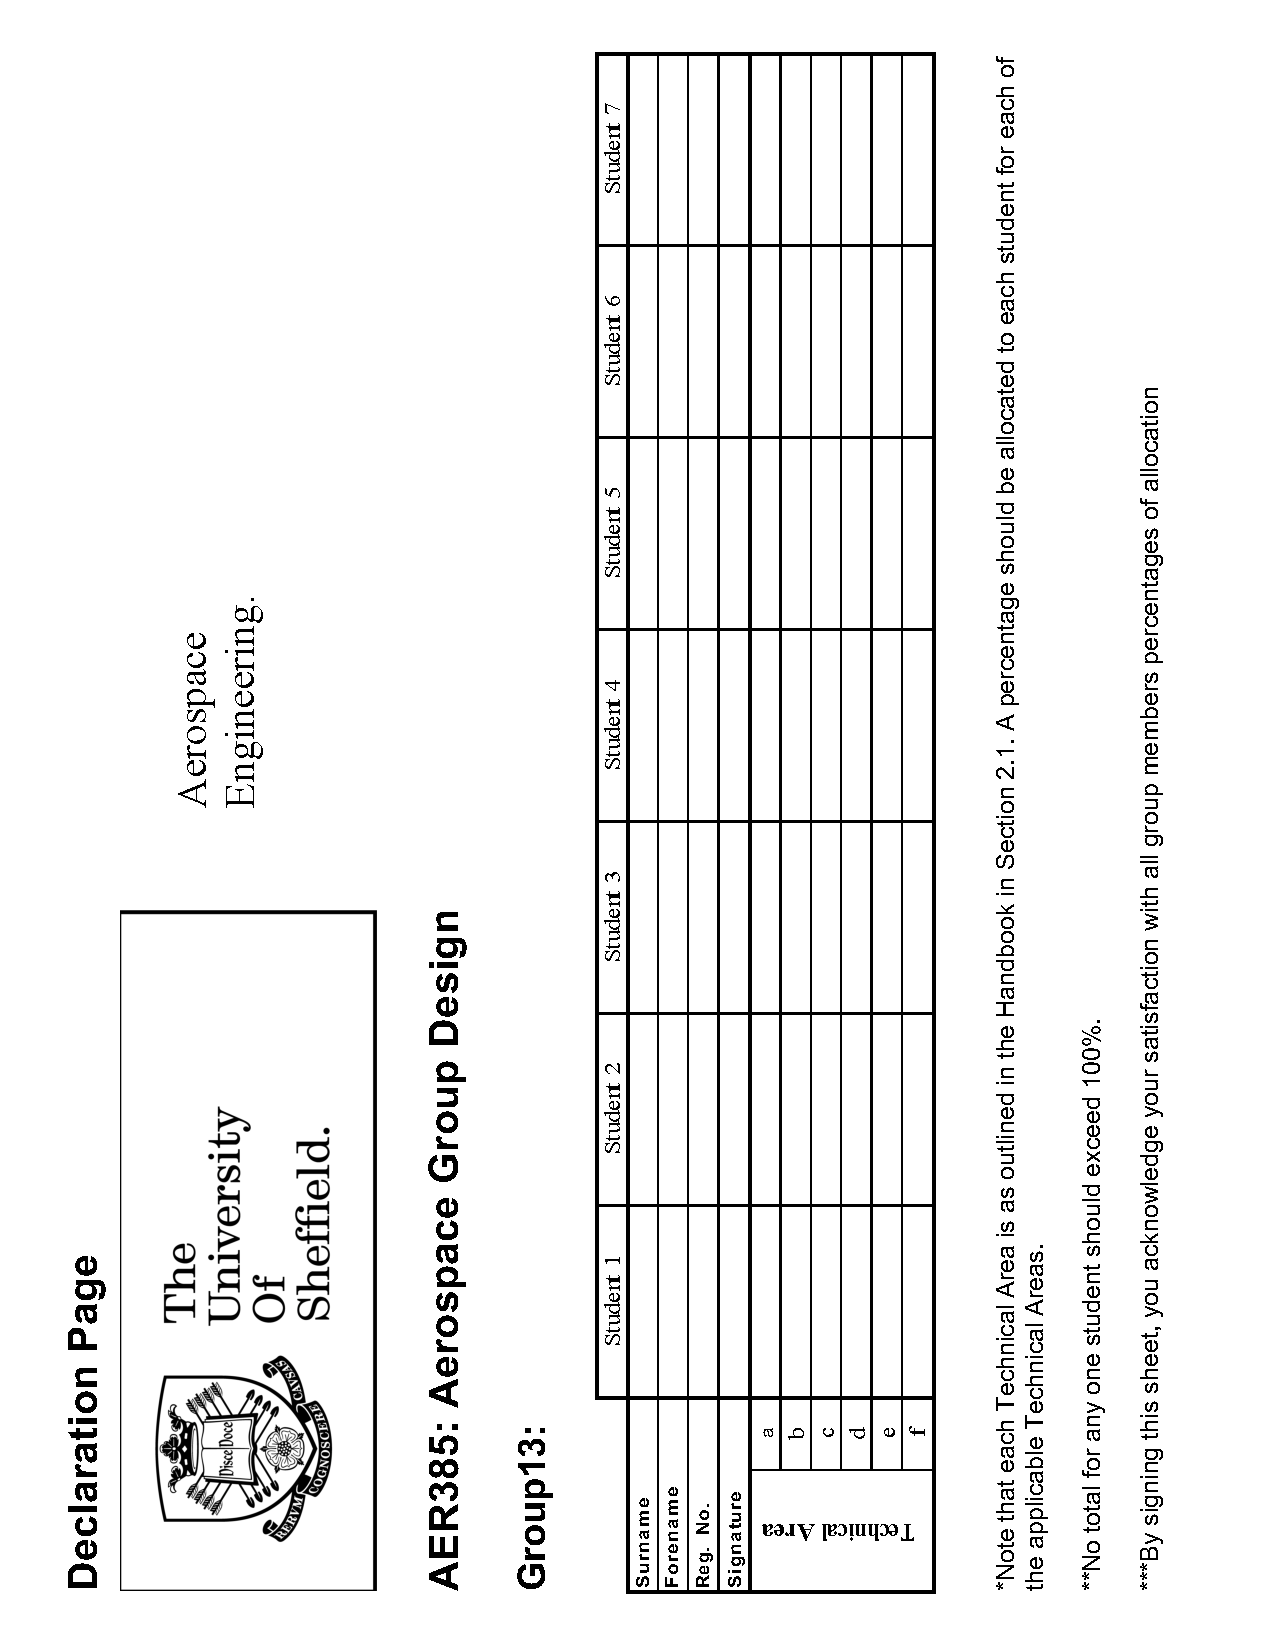
\includepdf[pages=-]{AER385.pdf}

\tableofcontents

\newpage

\section{Aims and Objectives}

\newpage

\section{Project Planning}

\subsection{Work Breakdown Structure}
\subsubsection{An Introduction to the Team}

\setlength\arrayrulewidth{0.7pt}
\begin{table}[!htpb]
    \begin{tabular}{ |p{3cm}|p{9cm}| }
        \hline
        \multicolumn{2}{|c|}{\textbf{Thomas Osland}} \\
        \hline
        & \makecell[tl]{\textbf{Role:} \\ \textbf{Description:}} \\
        \hline
        \multicolumn{2}{|c|}{\textbf{Ana-Maria Badilita}} \\
        \hline
        & \makecell[tl]{\textbf{Role:} \\ \textbf{Description:}} \\
        \hline
        \multicolumn{2}{|c|}{\textbf{Hamza Bouhouch}} \\
        \hline
        & \makecell[tl]{\textbf{Role:} \\ \textbf{Description:}} \\
        \hline
        \multicolumn{2}{|c|}{\textbf{Arthur Cunningham}} \\
        \hline
        & \makecell[tl]{\textbf{Role:} \\ \textbf{Description:}} \\
        \hline
        \multicolumn{2}{|c|}{\textbf{Tobias Sandin}} \\\hline
        & \makecell[tl]{\textbf{Role:} \\ \textbf{Description:}} \\
        \hline
        \multicolumn{2}{|c|}{\textbf{Samuel Vazquez}} \\
        \hline
        & \makecell[tl]{\textbf{Role:} \\ \textbf{Description:}} \\
        \hline
        \end{tabular}
    \captionof{table}{Group13 Team Members Profiles}
\end{table}

\newpage

\subsubsection{Schedule}

The project can be divided into 2 main phases; the table below shows the target tasks for the present semester and the current status of the key activities that are currently finalised, in progress or up-coming. 
The Ganntt Chart below explains some of the key activities taking place during the current stage and the people in charge of them.

\newpage 

\begin{figure}[hp]
    \centering
    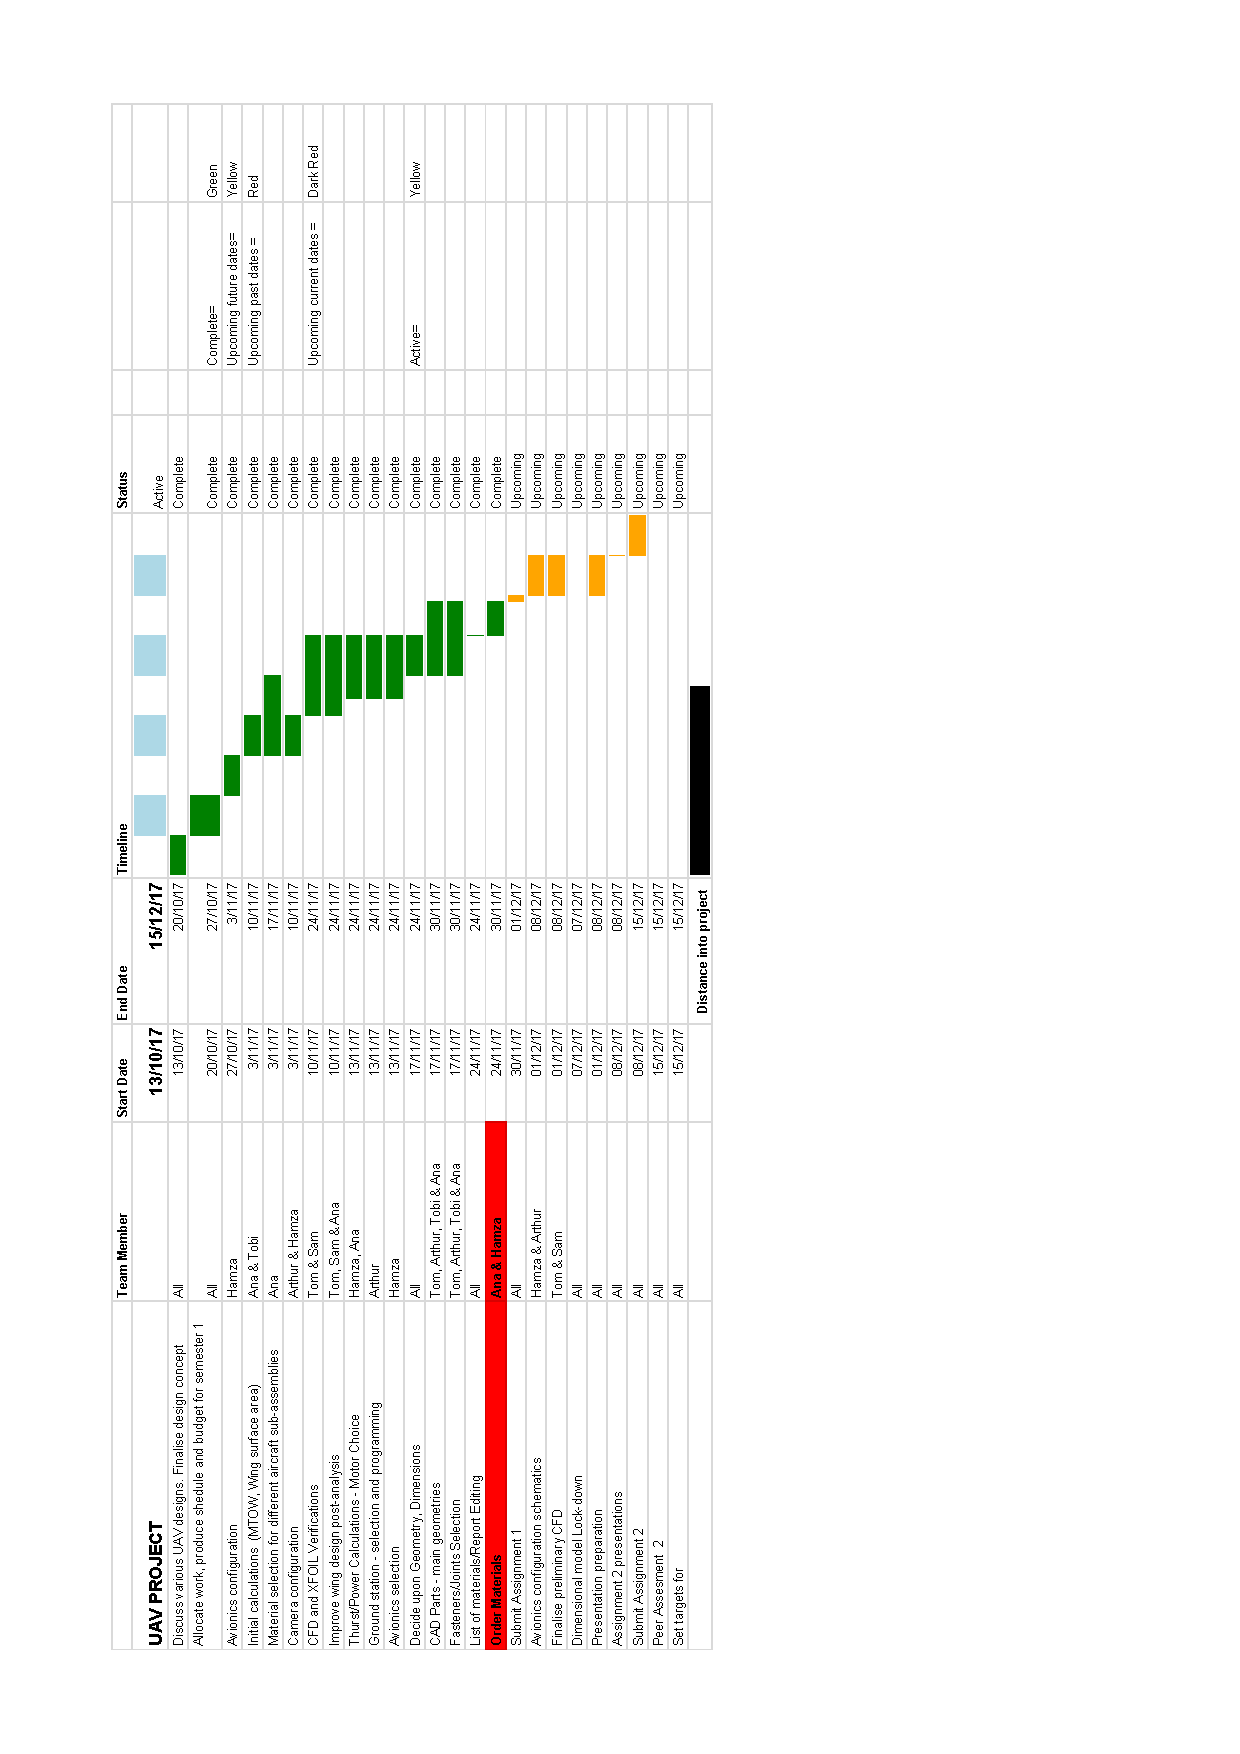
\includepdf[pages=-,scale=0.8,pagecommand={\thispagestyle{plain}\null\vfill}]{Gannt_Chart.pdf}
\end{figure}

\newpage

\subsection{Budget}

\newpage

\section{Initial Design}

\subsection{Conceptual Design}

\newpage

\subsection{Preliminary Design Review}

\subsubsection{Aerodynamics}

\subsubsection{Propulsion and Electrical Power}

\subsubsection{Materials and Structure}

\subsubsection{Ground Station and Communication}

\subsubsection{Control - Autopilot\textbackslash Autostabilisation}

\subsubsection{Sensors, Actuators and Communicators}

\newpage

\section{Conlusions Upon the Preliminary Design}

\newpage

\appendix

\section{Apendix }

\end{document}